\documentclass[12pt]{article}
\usepackage{graphicx}
\usepackage{amsmath}
\usepackage{mathtools}
\usepackage{gensymb}

\newcommand{\mydet}[1]{\ensuremath{\begin{vmatrix}#1\end{vmatrix}}}
\providecommand{\brak}[1]{\ensuremath{\left(#1\right)}}
\providecommand{\norm}[1]{\left\lVert#1\right\rVert}
\newcommand{\solution}{\noindent \textbf{Solution: }}
\newcommand{\myvec}[1]{\ensuremath{\begin{pmatrix}#1\end{pmatrix}}}
\let\vec\mathbf

\begin{document}
\begin{center}
\textbf\large{CHAPTER-11 \\ CIRCLES}

\end{center}
\section*{Excercise 11.1}

Q2.Find the equation of the circle with centre $(-2,3)$ and radius 4.

\solution
\\
Given
\begin{align}
	\vec{c} = \myvec{-2\\3} \text{ and } r = 4
\end{align}
The equation of the circle is given as
\begin{align}
	\norm{\vec{x}}^{2} + 2\vec{u}^{\top}\vec{x} + f = 0
\end{align}
Where,
\begin{align}
	\vec{u} &= -\vec{c} \text{ and } f = \norm{\vec{u}}^{2} - r^{2}\\
	\vec{u} &= \myvec{2\\-3},\norm{\vec{u}} = \sqrt{13}\\
	f &= \norm{\vec{u}}^2 - r^2\\
	&= (\sqrt{13})^2 - 4^2= -1
\end{align}
Now substituting the values the equation of circle can be given as
\begin{align}
	\norm{\vec{x}}^2 + 2\vec{u}^\top\vec{x}-1 &= 0\\
	\norm{\vec{x}}^2 + 2\vec{u}^\top\vec{x} &= 1\\
	\text{ where } \vec{u} = \myvec{2\\-3}        		       
\end{align}	
\begin{figure}[!h]
	\begin{center} 
	    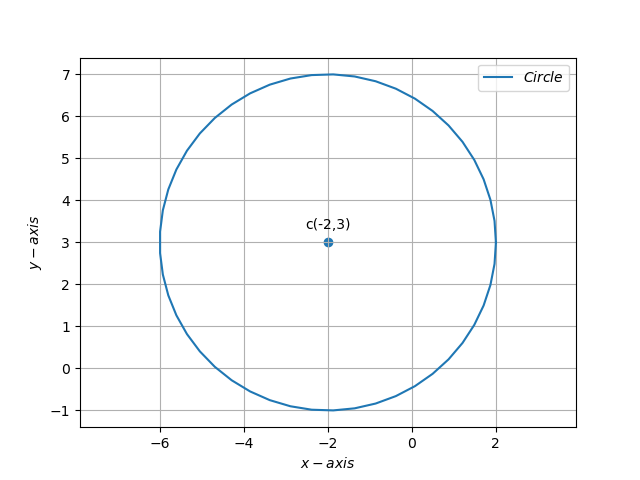
\includegraphics[width=\columnwidth]{figs/circle.png}
	\end{center}
\caption{}
\label{fig:Fig1}
\end{figure}

\end{document}
